% Final Project

\documentclass[a4paper, 12pt, notitlepage]{report}

\usepackage{amsfonts} % if you want blackboard bold symbols e.g. for real numbers
\usepackage{graphicx} % if you want to include jpeg or pdf pictures
\usepackage{multirow}
\usepackage{array}
\usepackage{cite}
\usepackage{amssymb}
\usepackage{amsmath}

\title{\textbf{Unit Commitment Problem}\\[2em]ECE619 Project Final Report}
\author{Jiahui Guo}
\date{May.6 2013}

\begin{document}

%%%%%%%%%% PRELIMINARY MATERIAL %%%%%%%%%%
\maketitle
\begin{center}
Supervised by Dr.\ Kevin Tomsovic.
\end{center}
\thispagestyle{empty}
\newpage
\section*{Acknowledgement of Sources}
For all ideas taken from other sources (books, articles, internet), the source of the ideas is mentioned in the main text and fully referenced at the end of the report.

All material which is quoted essentially word-for-word from other sources is given in quotation marks and referenced.

Pictures and diagrams copied from the internet or other sources are labelled with a reference to the web page or book, article etc.

\tableofcontents

%%%%%%%%%% MAIN TEXT STARTS HERE %%%%%%%%%%

%%%%%%%%%% SAMPLE CHAPTER %%%%%%%%%%
\chapter{Overall Problem Definition}
%


\section{Background}
%
Unit Commitment(UC) schedules the on-and-off times of the generating units, and calculates the minimum cost hourly generation schedule while ensuring that start-up and shut-down rates, minimum up and minimum down times are considered.\\
The UC is important because it is not only a way to promote the system economy, but also for the following reasons:\cite{1}
\begin{enumerate}
\item[1)]Start-up, shut-down and the dynamic considerations in restarting the modern generating facilities are much more complex and costier than they were for smaller, older units;
\item[2)]Growth in system size to the point where even small percentage gains have becomes economically very important;
\item[3)]Increase in variation between the peak and off-peak power demands;
\item[4)]System planning requires automated computerized schedulers to simulate the effect of unit selection methods on the choice of new generation;
\item[5)]Scheduling problem has grown out of the effective reach of the "earlier" techniques because of the large variaty in efficiencies and types of power sources.
\end{enumerate}

\section{Problem Definition}
%
In current system operation center, day-ahead schedule(Unit Commitment) and real-time balancing (Optimal Power Flow) are considered separately. In day-ahead schedule, ISOs schedule the startup and shutdown state and the power output of each generator for each time interval in order to minimize the overall cost over the next $24$ hours. In real time schedule, ISOs re-adjust each generator's output to balance demand and generation. This study only focuses on day-ahead UC problem.
In this project, a single bus system with 4 generators and one aggregated load is proposed. The constraints listed as following are added at different stages in order to solve the problem from simplicity to complexity.

\section{Modeling in Unit Commitment}

\subsection{Nomenclature}
\begin{description}
\item[$k$]Index for unit.
\item[$t$]Index for hour.
\item[$N_h$]Total hour horizon scheduled.
\item[$N_g$]Number of generator units.
\item[$P_k(t)$]Amount of electricity generated by generator $k$ in time period $t$.
\item[$Fs_{k}$]Half of start-up cost plus shut down cost.
\item[$D(t)$]Forecasted system demand at time $t$.
\item[$P_{min,k}$]Lower limit of real power generation of unit $k$.
\item[$P_{max,k}$]Upper limit of real power generation of unit $k$.
\item[$R(t)$]Amount of spinning reserve at time $t$.
\item[$Z_k(t)$]Binary variable to indicate if generator $k$ is on in time period $t$.
\item[$a_k,b_k,c_k$]Quadratic energy cost coefficients of unit $k$.
\end{description}

\subsection{Modeling}
\begin{gather}
\min\sum_{t=1}^{N_h} \sum_{k=1}^{N_g}[a_{k}(t)+b_{k}P_{k}(t)+c_{k}P_{k}^2(t)+Fs_{k}(1-Z_{k}(t-1))]Z_{k}(t)\label{eqn:equ1}
\end{gather}
\textit{s.t.} \\
\begin{gather}
\sum_{k=1}^{N_g}P_{k}(t) = D(t)\label{eqn:equ4}\\
P_{min,k}(t)Z_{k}(t)\leq P_{k}(t)\leq P_{max,k}(t)Z_{k}(t) \label{eqn:equ7}\\
P_{k}(t)+R_{k}(t)-\sum_{k=1}^{N_g}P_{max,k}Z_{k}(t)\leq 0\label{eqn:equ2}\\
Z_{k}(t)\in \{0,1\}\\
\forall k = 1,2,...,N_g\\
\forall t = 1,2,...,N_h
\end{gather}

\chapter{Solving the UC Problem}
\section{Approaches}
To solve the UC problem, there are various methods, classified as classical, non-classical and hybrid model\cite{2,3}. In this project, the following methods are utilized, the differences are the number of constraints considered when solving the UC problem.
\begin{enumerate}
\item[1)]Priority List
\item[2)]Dynamic Programming
\item[3)]Dynamic Programming + Priority List
\item[4)]Particle Swarm Optimization
\end{enumerate}

\subsection{Priority List}
The priority list is created according to each unit parameters. In this project, priority list is based on fuel cost
obtained from the average fuel cost of each unit operating at its maximum output power. The average full-load cost $\alpha$
is defined as the cost per unit of power \$\/MW when the unit is at its full capacity. It can be expressed as
\begin{equation}
\alpha_{i}=\frac{f_{i}(P_{max,i})}{P_{max,i}}+b_{i}+c_{i}P_{max,i}
\end{equation}
The units are ranked by their $\alpha$ in ascending order. Thus, the priority list of units will be formulated based on the order of $\alpha_{i}$,
in which a unit with the lowest $\alpha_{i}$ will have the highest priority to be dispatched.\cite{7}

\subsection{Dynamic Programming}
For the dynamic programming, it is a methodical procedure which systematically evaluates a large number of possible decisions in a multi-step problem. The convention dynamic programming takes all the states into account, for a $N_g$ generation, $N_h$ hours UC scheduling, the total path is ($2^{N_{g}}-1)^{N_{h}}$. In this project, the forward approach is utilized, the recursive algorithm is used to compute the minimum cost in hour $t$ with feasible state $I$, i.e.
\begin{equation}
F_{t,I}=\min[F(t,I)+S_{c}(t-1,L=>t,I)+F_{tc}(t-1,I)
\end{equation}
Where $F_{tc}(t,I)$ is the cost from initial state to hour $t$ state $I$, $S_{c}(t-1,L=>t,I)$ is the transition cost from state $(t-1,L)$ to state $(t,I)$, and $F(t,I)$ is the production cost for state $(t,I)$.
\subsection{Dynamic Programming + Priority List}
Since the priority list can have to choose better feasible states, for the dynamic programming, it doesn't have to traverse all the states, but only the feasible states filtered by priority list. And this method could promote the performance of dynamic programming.\cite{5}
\subsection{Particle Swarm Optimization}
PSO algorithm exploits a population of individuals(particles) to probe promising regions of search space, and each particle moves with an adaptable velocity within the regions of decision space and retains a memory of the best position it ever encountered. The best position ever attained by each particle of the swarm is communicated to all other particles.
The PSO assumes that the swarm is manipulated by the equation:
\begin{equation}
V_{i}^{t} = \omega V_{i}^{t-1}+C_{1}\cdot rand_{1}\cdot(P_{bi}^{t-1}-X_{i}^{t-1})+ C_{2}\cdot rand_{2}\cdot(P_{gbi}^{t-1}-X_{i}^{t-1})
\end{equation}
where
\begin{itemize}
  \item $\omega$: The inertia weight
  \item $C_{1},C_{2}$: The acceleration coefficients
  \item $rand_{1},rand_{2}$: Separately generated uniformed distributed random numbers between 0 and 1
  \item $X_{i}$: The position of the particle
  \item $V_{i}$: The velocity of the $ith$ dimension
\end{itemize}
And the $X_{i}^{t}$ is updated based on the velocity, since the $X_{i}^{t}$ should be a binary, a sigmoid function is applied to the velocity to produce a threshold, as follows:
\begin{equation}
rand() < sigmoid(V_{i})~? ~1~:~0
\end{equation}
The fitness function takes the reserve into consideration, and associates a penalty with the unbalance, as shown below:
\begin{eqnarray}
fitness(P_{k}(t)) &=& \sum_{t=1}^{N_h} \{\sum_{k=1}^{N_g}[a_{k}(t)+b_{k}P_{k}(t)+c_{k}P_{k}^2(t)+Fs_{k}(1-Z_{k}(t-1))]Z_{k}(t)\nonumber\\
&+&\lambda \cdot C \cdot((D(t)+R(t)-\sum_{k=1}^{N_g}P_{max,k}Z_{k})^{2}\}
\end{eqnarray}
where
\begin{itemize}
  \item $C$: A flag which used to indicate whether the constraint is violated, if so, $C=1$, otherwise, $C=0$.
  \item $\lambda$: The penalty coefficient.
\end{itemize}
The parameters in PSO should be carefully tuned, e.g. if the inertia weight is large, it benefits global search, while it is small, it is good at local search. In this project, a self-adjust weight is used as shown in the following equation.
\begin{equation}
\omega = \omega_{max} - \frac{(\omega_{max}-\omega_{min})\cdot iter}{MaxIter}
\end{equation}
Also, the larger $C_1$ may cause the particle converge to a local optimal, while larger $C_2$ may cause the particle converge to a global optimal.
The detailed parameters are obtained from \cite{8}.

\section{Data and Parameters}
The Generation data and load data are obtained from \cite{4}, as shown in Table \ref{table:table1} and Table \ref{table:table2}.
\begin{enumerate}
\item[1)]Generation Data
\item[2)]Load Data
\end{enumerate}

\begin{table}
\centering
\begin{tabular}{ | c | c || c | c || c | c || c | c |}
\hline
Hour & P$_{load}$ & Hour & P$_{load}$  & Hour & P$_{load}$ & Hour & P$_{load}$\\
\hline
1 & 480  & 2 & 530 & 3 & 600 & 4 & 540\\
\hline
5 & 400  & 6 & 280 & 7 & 290 & 8 & 500\\
\hline
\end{tabular}
\caption{Load data}
\label{table:table1}
\end{table}

\begin{table}
\centering
\begin{tabular}{|c|c|c|c|c|c|c|c|}
\hline
Generation. & P$_{max}$ & P$_{min}$ & Start Cost & Initial State & Coef$_{a}$ & Coef$_{b}$  &  Coef$_{c}$  \\
No.         & (MW)    & (MW)       & Cold(\$)  & at time 0     &     \$     &  \$/MWh  & \$/MWh$^{2}$ \\
\hline
1 & 80  & 25 & 350 & -5 & 970 & 17.26 & 0.0031\\
\hline
2 & 250 & 60 & 400 & 8  & 700 & 16.60 & 0.0020\\
\hline
3 & 300 & 75 & 600 & 8  & 680 & 16.50 & 0.0021\\
\hline
4 & 60  & 20 & 500 & -6 & 800 & 19.70 & 0.0039\\
\hline
\end{tabular}
\caption{Generator data}
\label{table:table2}
\end{table}

\chapter{Results}
The test system:
\begin{itemize}
  \item 4 Generation
  \item 8 hour UC scheduling.
\end{itemize}
The detailed scheduling results from these algorithms are listed in below sections, respectively.
\section{Priority List}
\begin{verbatim}
		Solving Using Priority List Method.
*******************************************************************

		UNIT COMMITMENT DETAILS IN EACH HOUR.


HOUR:  1             Load:  480.0 MW           TotalCost: $9560.0
-------------------------------------------------------------------
UNITS          ON/OFF         GENERATION     MIN MW         MAX MW
  1               0             0.0            0.0            0.0
  2               1           233.7           60.0          250.0
  3               1           246.3           75.0          300.0
  4               0             0.0            0.0            0.0
-------------------------------------------------------------------
TOTAL:            2           480.0          135.0          550.0


HOUR:  2             Load:  530.0 MW           TotalCost: $19999.6
-------------------------------------------------------------------
UNITS          ON/OFF         GENERATION     MIN MW         MAX MW
  1               0             0.0            0.0            0.0
  2               1           250.0           60.0          250.0
  3               1           280.0           75.0          300.0
  4               0             0.0            0.0            0.0
-------------------------------------------------------------------
TOTAL:            2           530.0          135.0          550.0


HOUR:  3             Load:  600.0 MW           TotalCost: $32982.6
-------------------------------------------------------------------
UNITS          ON/OFF         GENERATION     MIN MW         MAX MW
  1               1            68.3           25.0           80.0
  2               1           250.0           60.0          250.0
  3               1           281.7           75.0          300.0
  4               0             0.0            0.0            0.0
-------------------------------------------------------------------
TOTAL:            3           600.0          160.0          630.0


HOUR:  4             Load:  540.0 MW           TotalCost: $43599.3
-------------------------------------------------------------------
UNITS          ON/OFF         GENERATION     MIN MW         MAX MW
  1               0             0.0            0.0            0.0
  2               1           250.0           60.0          250.0
  3               1           290.0           75.0          300.0
  4               0             0.0            0.0            0.0
-------------------------------------------------------------------
TOTAL:            2           540.0          135.0          550.0


HOUR:  5             Load:  400.0 MW           TotalCost: $51763.0
-------------------------------------------------------------------
UNITS          ON/OFF         GENERATION     MIN MW         MAX MW
  1               0             0.0            0.0            0.0
  2               1           192.7           60.0          250.0
  3               1           207.3           75.0          300.0
  4               0             0.0            0.0            0.0
-------------------------------------------------------------------
TOTAL:            2           400.0          135.0          550.0


HOUR:  6             Load:  280.0 MW           TotalCost: $57227.7
-------------------------------------------------------------------
UNITS          ON/OFF         GENERATION     MIN MW         MAX MW
  1               0             0.0            0.0            0.0
  2               0             0.0            0.0            0.0
  3               1           280.0           75.0          300.0
  4               0             0.0            0.0            0.0
-------------------------------------------------------------------
TOTAL:            1           280.0           75.0          300.0


HOUR:  7             Load:  290.0 MW           TotalCost: $62869.3
-------------------------------------------------------------------
UNITS          ON/OFF         GENERATION     MIN MW         MAX MW
  1               0             0.0            0.0            0.0
  2               0             0.0            0.0            0.0
  3               1           290.0           75.0          300.0
  4               0             0.0            0.0            0.0
-------------------------------------------------------------------
TOTAL:            1           290.0           75.0          300.0


HOUR:  8             Load:  500.0 MW           TotalCost: $73180.4
-------------------------------------------------------------------
UNITS          ON/OFF         GENERATION     MIN MW         MAX MW
  1               0             0.0            0.0            0.0
  2               1           243.9           60.0          250.0
  3               1           256.1           75.0          300.0
  4               0             0.0            0.0            0.0
-------------------------------------------------------------------
TOTAL:            2           500.0          135.0          550.0

*******************************************************************

 The Optimal Total Cost is $73180.3876.
 Elapsed time:     0.0193 sec.

\end{verbatim}


\clearpage
\section{Dynamic Programming}
\begin{verbatim}
		Solving Using Dynamic Programming.
*******************************************************************
Starting processing the UC in hour 1
Starting processing the UC in hour 2
Starting processing the UC in hour 3
Starting processing the UC in hour 4
Starting processing the UC in hour 5
Starting processing the UC in hour 6
Starting processing the UC in hour 7
Starting processing the UC in hour 8

Processing Done!
*******************************************************************

		UNIT COMMITMENT DETAILS IN EACH HOUR.


HOUR:  1             Load:  480.0 MW           TotalCost: $9560.0
-------------------------------------------------------------------
UNITS          ON/OFF         GENERATION     MIN MW         MAX MW
  1               0             0.0            0.0            0.0
  2               1           233.7           60.0          250.0
  3               1           246.3           75.0          300.0
  4               0             0.0            0.0            0.0
-------------------------------------------------------------------
TOTAL:            2           480.0          135.0          550.0


HOUR:  2             Load:  530.0 MW           TotalCost: $19999.6
-------------------------------------------------------------------
UNITS          ON/OFF         GENERATION     MIN MW         MAX MW
  1               0             0.0            0.0            0.0
  2               1           250.0           60.0          250.0
  3               1           280.0           75.0          300.0
  4               0             0.0            0.0            0.0
-------------------------------------------------------------------
TOTAL:            2           530.0          135.0          550.0


HOUR:  3             Load:  600.0 MW           TotalCost: $32982.6
-------------------------------------------------------------------
UNITS          ON/OFF         GENERATION     MIN MW         MAX MW
  1               1            68.3           25.0           80.0
  2               1           250.0           60.0          250.0
  3               1           281.7           75.0          300.0
  4               0             0.0            0.0            0.0
-------------------------------------------------------------------
TOTAL:            3           600.0          160.0          630.0


HOUR:  4             Load:  540.0 MW           TotalCost: $43599.3
-------------------------------------------------------------------
UNITS          ON/OFF         GENERATION     MIN MW         MAX MW
  1               0             0.0            0.0            0.0
  2               1           250.0           60.0          250.0
  3               1           290.0           75.0          300.0
  4               0             0.0            0.0            0.0
-------------------------------------------------------------------
TOTAL:            2           540.0          135.0          550.0


HOUR:  5             Load:  400.0 MW           TotalCost: $51763.0
-------------------------------------------------------------------
UNITS          ON/OFF         GENERATION     MIN MW         MAX MW
  1               0             0.0            0.0            0.0
  2               1           192.7           60.0          250.0
  3               1           207.3           75.0          300.0
  4               0             0.0            0.0            0.0
-------------------------------------------------------------------
TOTAL:            2           400.0          135.0          550.0


HOUR:  6             Load:  280.0 MW           TotalCost: $57227.7
-------------------------------------------------------------------
UNITS          ON/OFF         GENERATION     MIN MW         MAX MW
  1               0             0.0            0.0            0.0
  2               0             0.0            0.0            0.0
  3               1           280.0           75.0          300.0
  4               0             0.0            0.0            0.0
-------------------------------------------------------------------
TOTAL:            1           280.0           75.0          300.0


HOUR:  7             Load:  290.0 MW           TotalCost: $62869.3
-------------------------------------------------------------------
UNITS          ON/OFF         GENERATION     MIN MW         MAX MW
  1               0             0.0            0.0            0.0
  2               0             0.0            0.0            0.0
  3               1           290.0           75.0          300.0
  4               0             0.0            0.0            0.0
-------------------------------------------------------------------
TOTAL:            1           290.0           75.0          300.0


HOUR:  8             Load:  500.0 MW           TotalCost: $73180.4
-------------------------------------------------------------------
UNITS          ON/OFF         GENERATION     MIN MW         MAX MW
  1               0             0.0            0.0            0.0
  2               1           243.9           60.0          250.0
  3               1           256.1           75.0          300.0
  4               0             0.0            0.0            0.0
-------------------------------------------------------------------
TOTAL:            2           500.0          135.0          550.0

*******************************************************************

 The Optimal Total Cost is $73180.3876.
 Elapsed time:     0.6517 sec.

\end{verbatim}


\clearpage
\section{Dynamic Programming + Priority List}
\begin{verbatim}
		Solving Using Dynamic Programming + Priority List Method.
*******************************************************************
Starting processing the UC in hour 1
Starting processing the UC in hour 2
Starting processing the UC in hour 3
Starting processing the UC in hour 4
Starting processing the UC in hour 5
Starting processing the UC in hour 6
Starting processing the UC in hour 7
Starting processing the UC in hour 8

Processing Done!
*******************************************************************

		UNIT COMMITMENT DETAILS IN EACH HOUR.


HOUR:  1             Load:  480.0 MW           TotalCost: $9560.0
-------------------------------------------------------------------
UNITS          ON/OFF         GENERATION     MIN MW         MAX MW
  1               0             0.0            0.0            0.0
  2               1           233.7           60.0          250.0
  3               1           246.3           75.0          300.0
  4               0             0.0            0.0            0.0
-------------------------------------------------------------------
TOTAL:            2           480.0          135.0          550.0


HOUR:  2             Load:  530.0 MW           TotalCost: $19999.6
-------------------------------------------------------------------
UNITS          ON/OFF         GENERATION     MIN MW         MAX MW
  1               0             0.0            0.0            0.0
  2               1           250.0           60.0          250.0
  3               1           280.0           75.0          300.0
  4               0             0.0            0.0            0.0
-------------------------------------------------------------------
TOTAL:            2           530.0          135.0          550.0


HOUR:  3             Load:  600.0 MW           TotalCost: $32982.6
-------------------------------------------------------------------
UNITS          ON/OFF         GENERATION     MIN MW         MAX MW
  1               1            68.3           25.0           80.0
  2               1           250.0           60.0          250.0
  3               1           281.7           75.0          300.0
  4               0             0.0            0.0            0.0
-------------------------------------------------------------------
TOTAL:            3           600.0          160.0          630.0


HOUR:  4             Load:  540.0 MW           TotalCost: $43599.3
-------------------------------------------------------------------
UNITS          ON/OFF         GENERATION     MIN MW         MAX MW
  1               0             0.0            0.0            0.0
  2               1           250.0           60.0          250.0
  3               1           290.0           75.0          300.0
  4               0             0.0            0.0            0.0
-------------------------------------------------------------------
TOTAL:            2           540.0          135.0          550.0


HOUR:  5             Load:  400.0 MW           TotalCost: $51763.0
-------------------------------------------------------------------
UNITS          ON/OFF         GENERATION     MIN MW         MAX MW
  1               0             0.0            0.0            0.0
  2               1           192.7           60.0          250.0
  3               1           207.3           75.0          300.0
  4               0             0.0            0.0            0.0
-------------------------------------------------------------------
TOTAL:            2           400.0          135.0          550.0


HOUR:  6             Load:  280.0 MW           TotalCost: $57227.7
-------------------------------------------------------------------
UNITS          ON/OFF         GENERATION     MIN MW         MAX MW
  1               0             0.0            0.0            0.0
  2               0             0.0            0.0            0.0
  3               1           280.0           75.0          300.0
  4               0             0.0            0.0            0.0
-------------------------------------------------------------------
TOTAL:            1           280.0           75.0          300.0


HOUR:  7             Load:  290.0 MW           TotalCost: $62869.3
-------------------------------------------------------------------
UNITS          ON/OFF         GENERATION     MIN MW         MAX MW
  1               0             0.0            0.0            0.0
  2               0             0.0            0.0            0.0
  3               1           290.0           75.0          300.0
  4               0             0.0            0.0            0.0
-------------------------------------------------------------------
TOTAL:            1           290.0           75.0          300.0


HOUR:  8             Load:  500.0 MW           TotalCost: $73180.4
-------------------------------------------------------------------
UNITS          ON/OFF         GENERATION     MIN MW         MAX MW
  1               0             0.0            0.0            0.0
  2               1           243.9           60.0          250.0
  3               1           256.1           75.0          300.0
  4               0             0.0            0.0            0.0
--------------------------------------------------------------------
TOTAL:            2           500.0          135.0          550.0

********************************************************************

 The Optimal Total Cost is $73180.3876.
 Elapsed time:     0.1860 sec.

\end{verbatim}


\clearpage
\section{Particle Swarm Optimization}
For the PSO, 10 times of execution are performed to obtain the best result, which are shown in Table \ref{table:table3}.

\begin{table}
\centering
\begin{tabular}{ | c | c || c | c || c | c || c | c || c | c |}
\hline
No. & Cost$_{min}$  & No. & Cost$_{min}$  & No. & Cost$_{min}$ & No. & Cost$_{min}$ & No. & Cost$_{min}$\\
\hline
1 & 80623.92  & 2 & 77172.67 & 3 & 80296.38 & 4 & 77172.67 & 5  & 77802.07\\
\hline
6 & 77207.24  & 7 & 77172.67 & 8 & 77172.67 & 9 & 77511.09 & 10 & 77172.67\\
\hline
\end{tabular}
\caption{PSO result}
\label{table:table3}
\end{table}

Some figures showing the iteration process of the PSO fitness function are shown in Figure \ref{Figure2}-\ref{Figure4}.

\begin{figure}
\centering
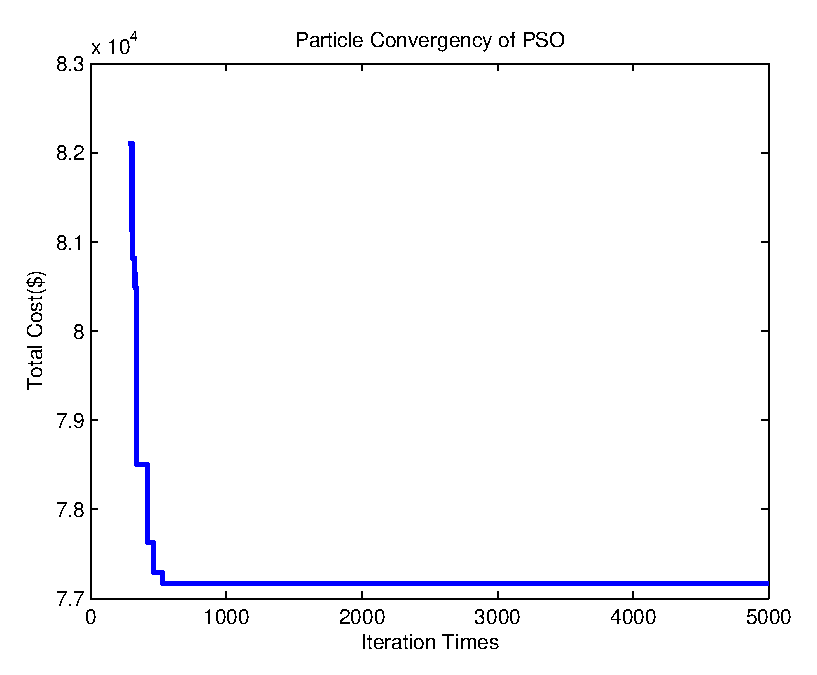
\includegraphics[height=0.6\textwidth]{2.eps}
\caption{PSO fitness function iteration (1).}
\label{Figure2}
\end{figure}

\begin{figure}
\centering
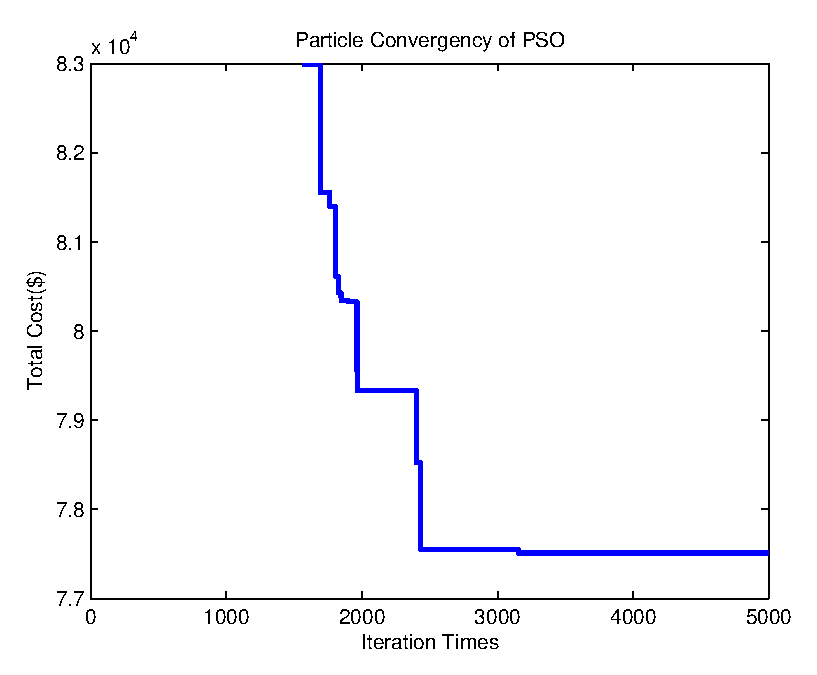
\includegraphics[height=0.6\textwidth]{9.eps}
\caption{PSO fitness function iteration (1).}
\label{Figure3}
\end{figure}

\begin{figure}
\centering
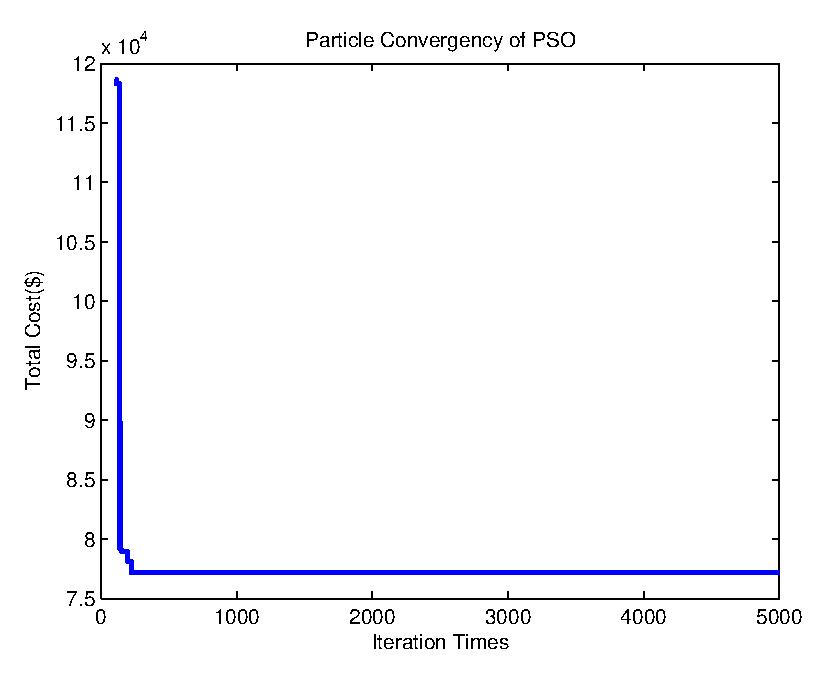
\includegraphics[height=0.6\textwidth]{10.eps}
\caption{PSO fitness function iteration (3).}
\label{Figure4}
\end{figure}

\clearpage
\begin{verbatim}
		Solving Using Particle Swarm Optimization.
*******************************************************************

		UNIT COMMITMENT DETAILS IN EACH HOUR.


HOUR:  1             Load:  480.0 MW           TotalCost: $10875.4
-------------------------------------------------------------------
UNITS          ON/OFF         GENERATION     MIN MW         MAX MW
  1               1            33.3           25.0           80.0
  2               1           216.6           60.0          250.0
  3               1           230.1           75.0          300.0
  4               0             0.0            0.0            0.0
-------------------------------------------------------------------
TOTAL:            3           480.0          160.0          630.0


HOUR:  2             Load:  530.0 MW           TotalCost: $22276.1
-------------------------------------------------------------------
UNITS          ON/OFF         GENERATION     MIN MW         MAX MW
  1               1            45.7           25.0           80.0
  2               1           235.9           60.0          250.0
  3               1           248.4           75.0          300.0
  4               0             0.0            0.0            0.0
-------------------------------------------------------------------
TOTAL:            3           530.0          160.0          630.0


HOUR:  3             Load:  600.0 MW           TotalCost: $34909.1
-------------------------------------------------------------------
UNITS          ON/OFF         GENERATION     MIN MW         MAX MW
  1               1            68.3           25.0           80.0
  2               1           250.0           60.0          250.0
  3               1           281.7           75.0          300.0
  4               0             0.0            0.0            0.0
-------------------------------------------------------------------
TOTAL:            3           600.0          160.0          630.0


HOUR:  4             Load:  540.0 MW           TotalCost: $46867.8
-------------------------------------------------------------------
UNITS          ON/OFF         GENERATION     MIN MW         MAX MW
  1               0             0.0            0.0            0.0
  2               1           250.0           60.0          250.0
  3               1           270.0           75.0          300.0
  4               1            20.0           20.0           60.0
-------------------------------------------------------------------
TOTAL:            3           540.0          155.0          610.0


HOUR:  5             Load:  400.0 MW           TotalCost: $55031.5
-------------------------------------------------------------------
UNITS          ON/OFF         GENERATION     MIN MW         MAX MW
  1               0             0.0            0.0            0.0
  2               1           192.7           60.0          250.0
  3               1           207.3           75.0          300.0
  4               0             0.0            0.0            0.0
-------------------------------------------------------------------
TOTAL:            2           400.0          135.0          550.0


HOUR:  6             Load:  280.0 MW           TotalCost: $60496.2
-------------------------------------------------------------------
UNITS          ON/OFF         GENERATION     MIN MW         MAX MW
  1               0             0.0            0.0            0.0
  2               0             0.0            0.0            0.0
  3               1           280.0           75.0          300.0
  4               0             0.0            0.0            0.0
-------------------------------------------------------------------
TOTAL:            1           280.0           75.0          300.0


HOUR:  7             Load:  290.0 MW           TotalCost: $67161.6
-------------------------------------------------------------------
UNITS          ON/OFF         GENERATION     MIN MW         MAX MW
  1               0             0.0            0.0            0.0
  2               1           136.3           60.0          250.0
  3               1           153.7           75.0          300.0
  4               0             0.0            0.0            0.0
-------------------------------------------------------------------
TOTAL:            2           290.0          135.0          550.0


HOUR:  8             Load:  500.0 MW           TotalCost: $77072.7
-------------------------------------------------------------------
UNITS          ON/OFF         GENERATION     MIN MW         MAX MW
  1               0             0.0            0.0            0.0
  2               1           243.9           60.0          250.0
  3               1           256.1           75.0          300.0
  4               0             0.0            0.0            0.0
-------------------------------------------------------------------
TOTAL:            2           500.0          135.0          550.0

*******************************************************************

 The Optimal Total Cost is $77172.6702.
 Elapsed time:   343.1562 sec.

\end{verbatim}



\clearpage
\section{The Optimization Result}
The optimization result from these methods are shown in Table \ref{table:table4}.
\begin{table}
\centering
\begin{tabular}{ | c | c | c | }
\hline
Algorithm & Cost(\$)  & Time(s)\\
\hline
PL    & 73180.39  & 0.0193\\
\hline
DP    & 73180.39  & 0.6517\\
\hline
DP+PL & 73180.39  & 0.1860\\
\hline
PSO   & 77172.67  & 343.15\\
\hline
\end{tabular}
\caption{Optimization result}
\label{table:table4}
\end{table}
\section{Observation}
\begin{itemize}
  \item The first three methods produce the same optimal solution, they all take the startup cost into consideration.
  \item Dynamic program needs more time than PL or DP+PL, since it needs to traverse more possible states.
  \item PSO considers the reserve constraint so that the optimal cost is higher than the other three.
\end{itemize}


\section{The Running Time Comparison}
The scale of the problem on time horizon is tested on $8h$, $16h$ and $24h$, it can be seen that the priority list, dynamic programming and their combination could produce almost linear runtime when the scheduling hour increase.  
\begin{figure}
\centering
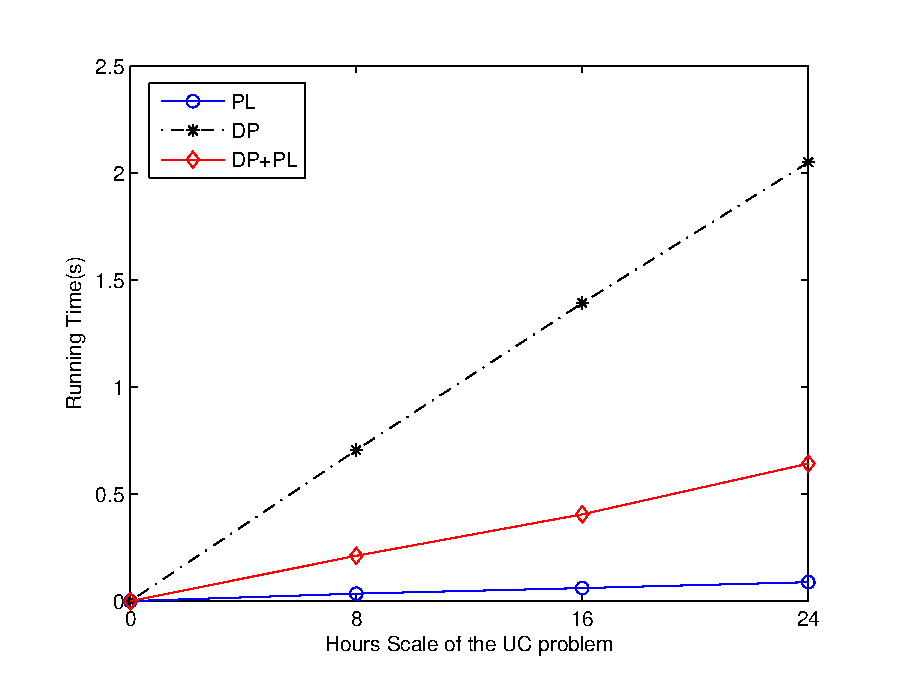
\includegraphics[height=0.6\textwidth]{runtime.eps}
\caption{Running Time comparison between DP and PL.}
\label{Figure1}
\end{figure}

%%%%%%%%%% APPENDIX %%%%%%%%%%
\appendix
\chapter{Source Code}
The hierarchy of the unit commitment solution code is shown as follows:
\begin{itemize}
  \item UC.m
  \item GetData.m
  \begin{itemize}
    \item PL
    \begin{itemize}
      \item PriorityList.m
    \end{itemize}
    \item DP
    \begin{itemize}
      \item PriorityList.m
      \item FeasibleStates.m
      \item Enumerate.m
    \end{itemize}
    \item PSO
    \begin{itemize}
      \item PSO.m
      \item fitness.m
      \item sigmoid.m
    \end{itemize}
  \end{itemize}
  \item UnitTest.m
  \item ED.m
  \item PrintResult.m
\end{itemize}

\section{Unit Commitment}
\begin{verbatim}
function UC()
tic
global FULLSTATES;
global DEBUG;
format long;

% Unit Test for each function, 1 means printing each function result
DEBUG = 0;

% Obtain the generation data and load data
[genData,loadData] = GetData();

% Choose an algorithm to solve
Algorithm = 1;

% Algorithm used to solve the UC problem
% 1: Priority List(PL)
% 2: Dynamic Programming(DP) + Full states
% 3: Dynamic Programming(DP) + Priorty lists
% 4: Particle Swarm Optimization(PSO)

switch Algorithm
    case 1
        fprintf('\n\t\tSolving Using Priority List Method.');
        fprintf('\n%s \n',repmat('*',1,100'));
        % No startup cost considered when scheduling
        OptimalCost = PL(genData,loadData);
    case 2
        % Startup cost considered
        FULLSTATES = 1;
        fprintf('\n\t\tSolving Using Dynamic Programming.');
        fprintf('\n%s \n',repmat('*',1,100'));
        OptimalCost = DP(genData,loadData);
    case 3
        FULLSTATES = 0;
        fprintf('\n\t\tSolving Using Dynamic Programming + ... 
                Priority List Method.');
        fprintf('\n%s \n',repmat('*',1,100'));
        OptimalCost = DP(genData,loadData);
        % Reserve requirement added
    case 4
        fprintf('\n\t\tSolving Using Particle Swarm Optimization.');
        fprintf('\n%s \n',repmat('*',1,100'));
        OptimalCost = PSO(genData,loadData);
    otherwise
        msgbox('Please specify a method!','WARNING!','warn');
end

t=toc;
fprintf('\n\n%s \n',repmat('*',1,100'));
fprintf('\n The Optimal Total Cost is $%10.4f.',OptimalCost);
fprintf('\n Elapsed time: %10.4f sec.\n\n',t)
\end{verbatim}

\section{Priority List}
\input{priorityList.tex}
\section{Dynamic Programming}
\begin{verbatim}
function OptimalCost = DP(G, Load)
% Dynamic programming

global FULLSTATES;

% Calculate the size of unit commitment problem
Nh = length(Load);               % # of load hour

if FULLSTATES == 0
    % Using Priority-list
    [States,GMax,GMin] = PriorityList(G);
else
    % Enumerate all the combinations
    [States,GMax,GMin] = Enumerate(G);
end

% Save N = 1 lowest cost for each transition

% Determine the initial state
IniState = (G.IniState > 0);
[~,IniStateId] = ismember(IniState,States','rows');

% Captitalized HOUR and STATE are indices
for HOUR = 1 : Nh
    fprintf('Starting processing the UC in hour %d\n', HOUR);

    % record the status of previous hour
    if HOUR == 1
        PreStateId = IniStateId;        % initial state
        PreTransM  = PreStateId;
    else
        PreFCost   = CurFCost;
        PreStateId = CurTransM(:,end);
        PreTransM  = CurTransM;
    end

    % Find all the feasible states for each hour(states index)
    [FeasiState, flag] = FeasibleStates(Load,GMax,GMin,HOUR,States);
    if (~flag)
        return;
    end

    NF = length(FeasiState);             % # of feasible states
    NP = length(PreStateId);             % # of previous states
    % Initialize the parameters
    % The total cost of getting to all feasible states in current hour
    CurFCost  = zeros(NF,1);
    % Transition matrix of optimal path to all feasible states in current hour
    CurTransM = zeros(NF,HOUR+1);
    % Total cost list for all previous states to a current state
    TotalCost = zeros(NP,1);
    % Search each feasible state
    for CurStateCnt = 1 : NF
        CurState = States(:,FeasiState(CurStateCnt));
        % Search each previous feasible state
        for PreStateCnt = 1 : NP
            if HOUR == 1
                PreState = IniState';
            else
                PreState = States(:,PreStateId(PreStateCnt));
            end
            % Check the state transition
            % stateTrans = 1 means commited, =1 means decommited
            StateTrans = CurState - PreState;
            % The start cost is cosidered as cold start
            GenStartCost = (StateTrans > 0)'.* G.Fsc;
            % For each feasible state, calculate the cost and dispatch
            [~,Cost] = ED(G.Coef_a,G.Coef_b,G.Coef_c,G.Pmax,G.Pmin,...
                        Load(HOUR),States(:,FeasiState(CurStateCnt)));
            if HOUR == 1
                TotalCost(PreStateCnt) = Cost + sum(GenStartCost);
            else
                TotalCost(PreStateCnt) = Cost + sum(GenStartCost)...
                                         + PreFCost(PreStateCnt);
            end
        end

        % Calculate the minimum cost to get to current state
        [CurFCost(CurStateCnt), Index] = min(TotalCost);
        % Update the transition matrix
        CurTransM(CurStateCnt,1:size(PreTransM,2)) = PreTransM(Index,:);
        CurTransM(CurStateCnt,end) = FeasiState(CurStateCnt);
    end
end
% End of search all the combination, then find the best path
[OptimalCost,Index] = min(CurFCost);
BestPath = CurTransM(Index,:);

fprintf('\nProcessing Done!');
fprintf('\n%s \n',repmat('*',1,100'));
% Print the UC result
PrintResult(G,Load,States(:,BestPath));
end
\end{verbatim}


\section{Particle Swarm Optimization}
\begin{verbatim}
function [OptimalCost,Pg] = PSO(G,Load)

% Setting the parameter for PSO
C1      = 2.02;        % Acceleration Coefficients
C2      = 2.05;
Xmin    = 0.0;         % Particle position limit
Xmax    = 1.0;
Wmin    = 0.2;         % The inertia weight limit
Wmax    = 1.0;
MaxIter = 5000;        % The maximum iteration times

% Solve the UC
NG = length(G.Pmin);    % # of generation
Nh = length(Load);      % # of load hour
X  = zeros(NG,Nh);      % The position of the particle(ON/OFF states)
V  = zeros(NG,Nh);      % Velocity of the i-th dimension
Pg = zeros(NG,Nh);      % Global best record
D  = 2^NG;              % Dimension of the search space

% The fitness objective
FITg = ones(MaxIter,1) * Inf;        % global best
FITp = ones(D,1) * Inf;              % personal best

% Define the swarm of the particle in the whole search space
S  = cell(2,D);                      % Current position
Pb = cell(1,D);                      % Personal best position

% Initialize the particles and velocity
for k = 1 : D
    for i = 1 : NG
        for j = 1 : Nh
            X(i,j) = randi([Xmin,Xmax]);        % random initialize position
            V(i,j) = Xmin + rand*(Xmax - Xmin); % random initialize velocity
        end
    end
    Pb{k}  = X;
    S{1,k} = X;
    S{2,k} = V;
end

% PSO iteration to search the global optimal objective
for iter = 1 : MaxIter
    w = Wmax - (Wmax - Wmin)*iter/MaxIter;      % inertial weight approach
    for k = 1 : D
        X = S{1,k};
        V = S{2,k};
        for i = 1 : NG
            for j = 1 : Nh
                % Update the velocity
                V(i,j) = w*V(i,j) + C1*rand*(Pb{k}(i,j)-X(i,j)) ... 
                         + C2*rand*(Pg(i,j)-X(i,j));

                % Using sigmoid function as a threshold
                if(rand < sigmoid(V(i,j)))
                    X(i,j) = 1;
                else
                    X(i,j) = 0;
                end
            end
        end

        % Update the current particle
        S{1,k} = X;
        S{2,k} = V;

        % Calculate the fitness for current particle
        FIT = fitness(G,Load,X);

        % Update the personal best position vector
        if FIT < FITp(k)
            FITp(k) = FIT;
            Pb{k} = X;
        end
    end

    % Update the global best position vector
    [FITg(iter), index] = min(FITp);
    Pg = Pb{index};
end

if FITg(iter) == Inf
    OptimalCost = Inf;
    fprintf('Not Converge!');
    %msgbox('PSO does not converge!','WARNING','warn');
    return;
end

% Plot the iteration of the optimal cost
figure;
plot(FITg,'LineWidth',2);
xlabel('Iteration Times');
ylabel('Total Cost($)');
title('Particle Convergency of PSO');

% Determine the initial state
IniState = (G.IniState > 0)';
States = [IniState,Pg];

% Print the scheduling result
PrintResult(G,Load,States);
OptimalCost = FITg(iter);

end
\end{verbatim}


\section{Economic Dispatch}
\begin{verbatim}
function [P, Cost] = ED(a,b,c,GMax,GMin,Load,state)
global DEBUG;
warning off %#ok<WNOFF>

state = logical(state);           % tranform to logical expression
% F(P) = a+b*P+c*P^2
NG = length(GMin);
P = zeros(NG,1);

lb = GMin(state);
ub = GMax(state);
H = 2*diag(c(state));
f = b(state);
Aeq = ones(1,NG);
Aeq = Aeq(state');
beq = Load;
options = optimset('Display','Off');
[Gen,Cost,exitflag] = quadprog(H,f,[],[],Aeq,beq,lb,ub,[],options);
if exitflag == 1
    Cost = Cost + a*state;
    P(state) = Gen;
else
    Cost = Inf;
    if DEBUG
        msg = ['No feasible dispatch for current combination: ', ...
                num2str(state'), '!'];
        msgbox(msg,'WARNING!','warn');
    end
    return;
end

end
\end{verbatim}


\section{Get Data}
\begin{verbatim}
function [G, L] = GetData()

L = [480;530;600;540;400;280;290;500];

G.Pmin    = [25,60,75,20];                        %MW
G.Pmax    = [80,250,300,60];                      %MW
G.Fsc     = [350,400,600,500];                    %Cold startup cost
G.Fsd     = [0,0,0,0];                            %Shut down cost
G.IniState= [-5,8,8,-6];                          %Init Condition

G.RampUp  = [50,80,100,80];                       %MW/h
G.RampDown= [75,120,150,120];                     %MW/h

G.Coef_a  = [970,700,680,800];                    %$
G.Coef_b  = [17.26,16.60,16.50,19.70];            %$/MWh
G.Coef_c  = [0.0031,0.0020,0.0021,0.0039];        %$/MWh^2
end
\end{verbatim}




\section{Generate All the States}
\begin{verbatim}
function [states,GMax,GMin] = Enumerate(G)
global DEBUG;

NG = length(G.Pmin);          % # of generation

% Generate the full states list, each column stands for a state
states = dec2bin(1:2^NG-1);
% tranform to logical expression
states = logical(sscanf(states,'%1d',size(states)));
GMax = states * G.Pmax';
GMin = states * G.Pmin';
states = states';

if DEBUG
    UnitTest(2,states,GMax,GMin);
end

end
\end{verbatim}


\section{Find Feasible States}
\begin{verbatim}
function [NStates, flag] = FeasibleStates(Load,GMax,GMin,HOUR,states)
global DEBUG;

NStates = find(Load(HOUR) <= GMax & Load(HOUR) >= GMin);
if isempty(NStates)
    flag = false;
    msg = ['No feasible states in hour ', num2str(HOUR), '!'];
    msgbox(msg,'No feasible states!','warn');
    return;
else
    flag = true;

    if DEBUG
        UnitTest(3,states(:,NStates),GMax(NStates),GMin(NStates));
    end
end
end
\end{verbatim}


\section{Sigmoid Function}
\begin{verbatim}
function y = sigmoid(x)
    y = 1/(1+exp(-x));
end
\end{verbatim}



\section{Unit Test}
\begin{verbatim}
function UnitTest(varargin)

if varargin{1} == 1             % Unit test for priority list states
    states = varargin{2};
    GMax = varargin{3};
    GMin = varargin{4};
    printStates(states,GMax,GMin);

elseif varargin{1} == 2          % Unit test for enumerate states
    states = varargin{2};
    GMax = varargin{3};
    GMin = varargin{4};
    printStates(states,GMax,GMin);

elseif varargin{1} == 3         % Unit test for feasible states search
    states = varargin{2};
    GMax = varargin{3};
    GMin = varargin{4};
    printStates(states,GMax,GMin);
end

function printStates(states,GMax,GMin)
NG = size(states,1);
fprintf('   State No.      MW min        MW max                     Units\n');
fprintf('%s',repmat(' ',1,23));
fprintf(['               ',repmat('    %5d ', 1, NG)],1:NG);
fprintf('\n %s \n',repmat('-',1,80'));
for i=1:size(states,2)
    fprintf('      %2d       %8.1f      %8.1f ',i,GMax(i),GMin(i));
    fprintf([repmat('       %2d ', 1, size(states,1)) '\n'], states(:,i));
end
fprintf('%s \n',repmat('-',1,80'));
end
\end{verbatim}


\section{Print Result}
\begin{verbatim}
function OptimalCost = PrintResult(G,Load,FullStates)

NG = length(G.Pmin);            % # of generations
Nh = length(Load);              % # of load hour
TotalCost = zeros(Nh,1);
CurState  = zeros(NG,Nh);
% Print
fprintf('\n\t\tUNIT COMMITMENT DETAILS IN EACH HOUR.');
for HOUR = 1 : Nh
    CurState(:,HOUR) = FullStates(:,HOUR+1);
    % Check the state transition
    % stateTrans = 1 means commited, =1 means decommited
    StateTrans = CurState(:,HOUR) - FullStates(:,HOUR);
    % The start cost is cosidered as cold start
    GenStartCost = (StateTrans > 0)'.* G.Fsc;
    GMin = CurState(:,HOUR).* G.Pmin';
    GMax = CurState(:,HOUR).* G.Pmax';
    [Generation,Cost] = ED(G.Coef_a,G.Coef_b,G.Coef_c,G.Pmax,G.Pmin,...
                           Load(HOUR),CurState(:,HOUR));
    if HOUR == 1
        TotalCost(HOUR) = Cost + sum(GenStartCost);
    else
        TotalCost(HOUR) = Cost + sum(GenStartCost) + TotalCost(HOUR-1);
    end
    S = ['UNITS          '
         'ON/OFF         '
         'GENERATION     '
         'MIN MW         '
         'MAX MW         '];
    TEMP = [(1:NG).',CurState(:,HOUR),Generation,GMin,GMax];
    fprintf('\n\n\nHOUR: %2d             Load:%7.1f MW           ...
            TotalCost: $%6.1f',HOUR,Load(HOUR),TotalCost(HOUR));
    fprintf('\n%s \n',repmat('-',1,100'))
    fprintf([repmat('%15s ', 1, size(S,1)) '\n\n'], S');fprintf('\n');
    fprintf(['%3d %15d ',repmat('%15.1f', 1, size(TEMP,2)-2) '\n'], TEMP.');
    fprintf('%s \n',repmat('-',1,100'));
    fprintf('TOTAL: %12d  %14.1f %14.1f %14.1f %14.1f %14.1f\n', ...
             sum(CurState(:,HOUR)),sum(Generation), sum(GMin), sum(GMax));
end
OptimalCost = TotalCost(end);
end
\end{verbatim}



\bibliography{IEEEabrv,bibfile}
\bibliographystyle{IEEEtran}

\end{document}
